\documentclass[aspectratio=169]{beamer}

\usetheme{default}

\usepackage[utf8]{inputenc}
\usepackage[russian]{babel}
\usepackage[OT1]{fontenc}
\usepackage{amsmath}
\usepackage{amsfonts}
\usepackage{amssymb}
\usepackage{graphicx}
\usepackage{etoolbox}
\usepackage{caption}
\usepackage{subcaption}
\captionsetup{compatibility=false}
\usepackage{pifont}
%\usepackage{subfigure}
\usepackage{xcolor}
\usepackage{framed}
\usepackage{empheq}
\usepackage[many]{tcolorbox}
\usepackage{multirow}
\usepackage{tikz}
\usepackage{listings}
\usepackage{tikz}

\definecolor{shadecolor}{cmyk}{0,0,0,1}

\lstset{
	backgroundcolor=\color{lightgray},
	commentstyle=\color{blue},
	frame=single
	breakatwhitespace, 
	language=python, 
	columns=fullflexible, 
	keepspaces, 
	breaklines, 
	tabsize=3, 
	showstringspaces=false, 
	extendedchars=true,
	numbers=left
}

\makeatletter

\setbeamercolor{title}{fg=white}
\setbeamercolor{frametitle}{fg=black}
\setbeamerfont*{title}{family=\sffamily,size=\LARGE}

\setbeamerfont{page number in head/foot}{size=\scriptsize}
\setbeamertemplate{footline}[frame number]
\let\otp\titlepage
\renewcommand{\titlepage}{\otp\addtocounter{framenumber}{-1}}

\setbeamertemplate{background canvas}{%
	\ifnumequal{\c@framenumber}{0}{%
		\vbox to \paperheight{\vfil\hbox to \paperwidth{\hfil
\includegraphics[height=\paperheight]{images/cover.png}\hfil}\vfil}
   }{%
      \ifnumequal{\c@framenumber}{\inserttotalframenumber}{
        \vbox to \paperheight{\vfil\hbox to \paperwidth{\hfil
\includegraphics[height=\paperheight]{images/back.png}\hfil}\vfil}
      }{%
         % Other frames
      }%
   }%
}

\makeatother

\beamertemplatenavigationsymbolsempty

\tcbset{highlight math style={enhanced,colframe=red,colback=white,arc=4pt,boxrule=1pt}}

\usetikzlibrary{shadings,shadows,shapes.arrows}

\newcommand*{\tikzarrow}[2]{%
  \tikz[
    baseline=(A.base),             % Set baseline to the baseline of node content
    font=\footnotesize\sffamily    % Set fontsize of the node content
  ]
  \node[
    single arrow,                  % Shape of the node
    single arrow head extend=5pt,  % Actual width of arrow head
    draw,                          % Draw the node shape
    inner sep=3pt,                 % Separation between node content and node shape
    top color=#1,               % Shading color on top of node
    bottom color=#1,               % Shading color on bottom of node
    % drop shadow                    % Draw a shadow
  ] (A) {#2};%
}

\newcommand{\tikzfancyarrow}[2][2cm]{\tikz[baseline=-0.5ex]\node [arrowstyle=#1] {#2};}
\newcommand*\rot{\rotatebox{90}}

\author{Николай Анохин}
\title{\newline \newline \newline Лекция 9 \\ Линейные модели \\ вероятностная перспектива}

\begin{document}

\begin{frame}[plain]
\titlepage
\end{frame}

\begin{frame}{План занятия}
\tableofcontents
\end{frame}

\begin{frame}{Постановка задачи}

{\bf Дано.} Признаковые описания $N$ объектов $\mathbf{x} = (x_1, \ldots, x_m) \in \mathcal{X}$, образующие тренировочный набор данных $X$, и значения целевой переменной $y = f(\mathbf{x}) \in \mathcal{Y}$ для каждого объекта из $X$. 

\vspace{1em}
{\bf Найти.} Для семейства параметрических функций 
\[
H = \{h(\mathbf{x, \mathbf{\theta}}) = y: \mathcal{X} \times \Theta \rightarrow \mathcal{Y}\},
\]
найти значение вектора параметров $\theta^*$, такое что $h^*(\mathbf{x}) = h(\mathbf{x}, \theta^*)$ наилучшим образом приближает целевую функцию.

\begin{eqnarray*}
Y & \in & \{C_1, C_2, \ldots, C_N\} \text{ -- задача классификации}  \\
Y & \in & [a, b] \subset \mathcal{R} \text{ -- задача регресии}
\end{eqnarray*}

\end{frame}

% ============================================== %

\section{Линейная регрессия}

% ============================================== %

\begin{frame}{}

\begin{center}
\Large Линейная регрессия

\vspace{1em}
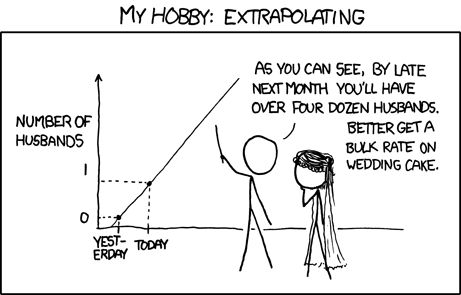
\includegraphics[height=0.7\textheight]{images/lr_joke.jpg}
\end{center}

\end{frame}

\begin{frame}{}

\begin{columns}[c]
    \begin{column}{.55\textwidth}
    	Модель
		\[
			y = h(\mathbf{x}, \theta) + \epsilon,
		\]
		где $\epsilon$ -- гауссовский шум
		\[
			p(\epsilon) = \mathcal{N}(\epsilon | 0, \beta^{-1}),
		\]
		откуда
		\[
		p(y | \mathbf{x}, \theta, \beta) = \mathcal{N}(y | h(\mathbf{x}, \theta), \beta^{-1}).
		\]
		Предсказание
		\[
		E[y | \mathbf{x}] = \int y p(y | \mathbf{x}) d y = h(\mathbf{x}, \theta).
 		\]
    \end{column}
       
    \begin{column}{.45\textwidth}
	\begin{center}
   		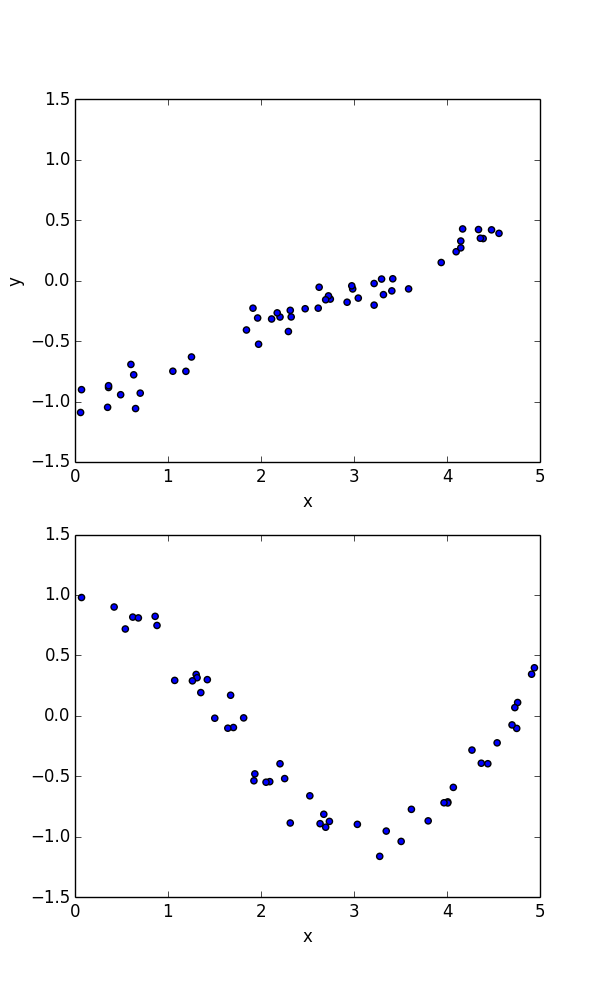
\includegraphics[scale=0.3]{images/empty_reg.png}
    \end{center}
    \end{column}
  \end{columns}

\end{frame}

\begin{frame}{Линейная модель}

\begin{columns}[c]
    \begin{column}{.55\textwidth}
    	простейшая модель
    	\[
    	h(\mathbf{x}, \mathbf{w}) = w_0 + w_1 x_1 + \ldots + w_M x_M = \sum_{j=0}^M w_j x_j
    	\]
    	улучшенная модель
    	\[
    	h(\mathbf{x}, \mathbf{w}) = \sum_{j=0}^M w_j \phi_j(\mathbf{x}) = \mathbf{w}^T \phi(\mathbf{x}),
    	\]
    	$\phi_j(\mathbf{x})$ -- базисные функции, $\phi_0(\mathbf{x}) = 1$ \\ \vspace{1em}
    	примеры
    	\[
    	\varphi_j(x) = x^j, \quad
    	\varphi_j(x) = \exp \left\{-\frac{(x - \mu_j)^2}{2 s^2} \right\}
    	\]
    \end{column}
       
    \begin{column}{.45\textwidth}
	\begin{center}
   		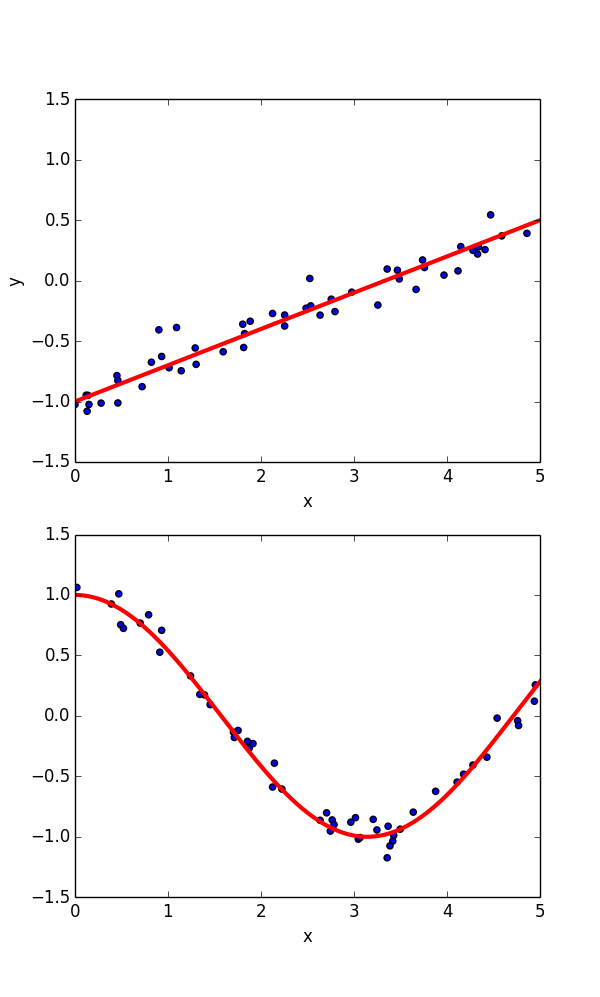
\includegraphics[scale=0.3]{images/full_reg.png}
    \end{center}
    \end{column}
  \end{columns}

\end{frame}

\begin{frame}{ML -- функция правдоподобия}

Дана обучающая выборка $\mathcal{D} = (X, Y)$ из $N$ объектов $(\mathbf{x_n}, y_n)$

\vspace{1em}
Функция правдоподобия
\[
\log p(Y | X, \mathbf{w}, \beta) = \sum_{n=1}^N \log \mathcal{N}(y | \mathbf{w}^T \phi(\mathbf{x_n}), \beta^{-1}) = 
\]
\[
= \frac{N}{2} \log \beta - \frac{N}{2} \log 2 \pi - \frac{\beta}{2} \sum_{n=1}^N \{y_n - \mathbf{w}^T \phi(\mathbf{x}_n)\}^2 \rightarrow \max_{\mathbf{w}, \beta}
\]
Квадратичная функция потерь
\[
E_D(\mathbf{w}) = \frac 1 2 \sum_{n=1}^N \{y_n - \mathbf{w}^T \phi(\mathbf{x}_n)\}^2 \rightarrow \min_{\mathbf{w}}
\]

\end{frame}

\begin{frame}{ML -- решение}

\[
\log p(Y | X, \mathbf{w}, \beta)
= \frac{N}{2} \log \beta - \frac{N}{2} \log 2 \pi - \frac{\beta}{2} \sum_{n=1}^N \{y_n - \mathbf{w}^T \phi(\mathbf{x}_n)\}^2 \rightarrow \max_{\mathbf{w}, \beta}
\]
Градиент
\[
\beta \sum_{n=1}^N \{y_n - \mathbf{w}^T \phi(\mathbf{x}_n)\} \phi(\mathbf{x_n})^T = 0
\]
Решение
 \[
 \mathbf{w}_{ML} = \mathbf{\Phi}^{\dagger} Y = (\mathbf{\Phi}^T \mathbf{\Phi})^{-1} \mathbf{\Phi}^T Y, \quad
 \frac{1}{\beta_{ML}} = \frac{1}{N} \sum_{n=1}^N \{y_n - \mathbf{w}_{ML}^T \phi(\mathbf{x}_n)\}^2, 
 \]
 где
 \[
 \mathbf{\Phi} = \begin{pmatrix}
 \phi_0(\mathbf{x_1}) & \ldots &  \phi_M(\mathbf{x_1}) \\
 \phi_0(\mathbf{x_2}) & \ldots &  \phi_M(\mathbf{x_2}) \\
 \ldots & \ldots & \ldots \\
  \phi_0(\mathbf{x_N}) & \ldots &  \phi_M(\mathbf{x_N}) \\
 \end{pmatrix}
 \]

\end{frame}

\begin{frame}{Регуляризация}

Функция потерь
\[
E(\mathbf{w}, \lambda) = E_D(\mathbf{w}) + \lambda E_W(\mathbf{w}),
\]
где (как и раньше)
\[
E_D(\mathbf{w}) = \frac 1 2 \sum_{n=1}^N \{y_n - \mathbf{w}^T \phi(\mathbf{x}_n)\}^2 \rightarrow \min_{\mathbf{w}},
\]
плюс регуляризация
\[
E_W(\mathbf{w}) = E_q(\mathbf{w}) = \sum_{j=1}^M |\mathbf{w}_j|^q
\]
Зоопарк
\begin{itemize}
\item $q = 1$ -- Lasso
\item $q = 2$ -- Ridge (байесовский вывод: $p(\mathbf{w} | \alpha) = \mathcal{N}(\mathbf{w} | 0, \alpha^{-1} \mathbf{I})$)
\item $E_W(\mathbf{w}) = \rho E_1(\mathbf{w}) + (1 - \rho) E_2(\mathbf{w})$ -- Elastic Net
\end{itemize}

\end{frame}

\begin{frame}{Робастная регрессия}

{\bf Проблема:} линейная регрессия чувствительна к шуму из-за того, что плотность нормального распределение очень быстро убывает

\vspace{1em}
{\bf Решения:}
\begin{itemize}
\item MAE вместо MSE
\item LTS: Least Trimmed Sum of Squares \footnote{\href{https://en.wikipedia.org/wiki/Least_trimmed_squares}{Least trimmed squares (wikipedia)}}
\item RANSAC \footnote{\href{https://en.wikipedia.org/wiki/RANSAC}{RANSAC (wikipedia)}}
\item t-Distribution вместо Гаусса
\end{itemize}

\end{frame}

% ============================================== %

\section{Логистическая регрессия}

% ============================================== %

\begin{frame}{}

\begin{center}
\Large Логистическая регрессия

\vspace{1em}
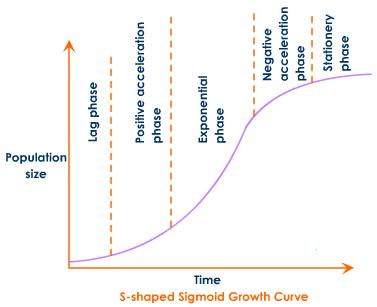
\includegraphics[height=0.7\textheight]{images/sigmoid-growth-curve.jpg}
\end{center}

\end{frame}

\begin{frame}{Ирисы Фишера}

\begin{center}
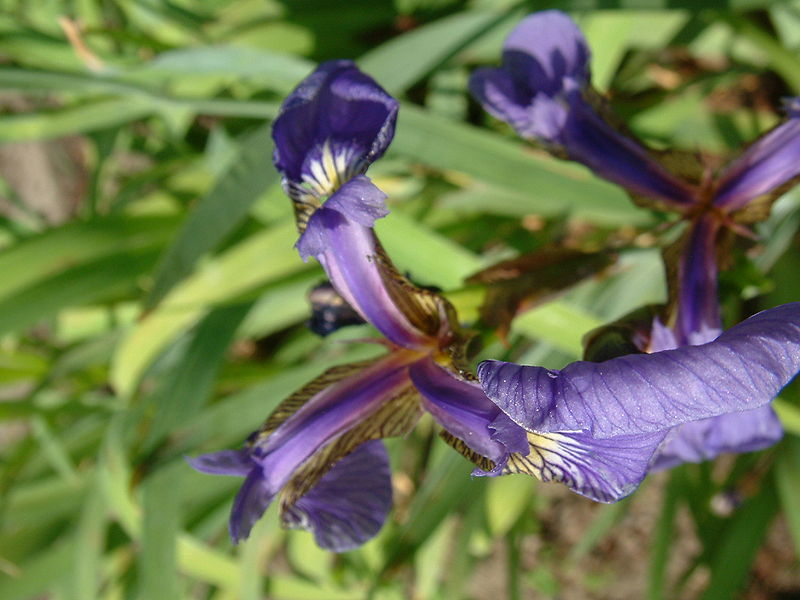
\includegraphics[scale=0.1]{images/setosa.jpg} \;
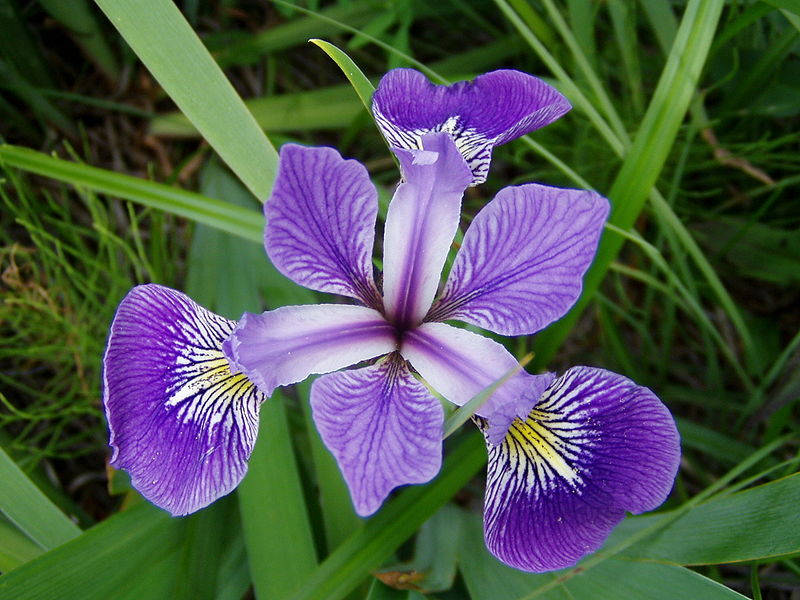
\includegraphics[scale=0.1]{images/versicolor.jpg} \;
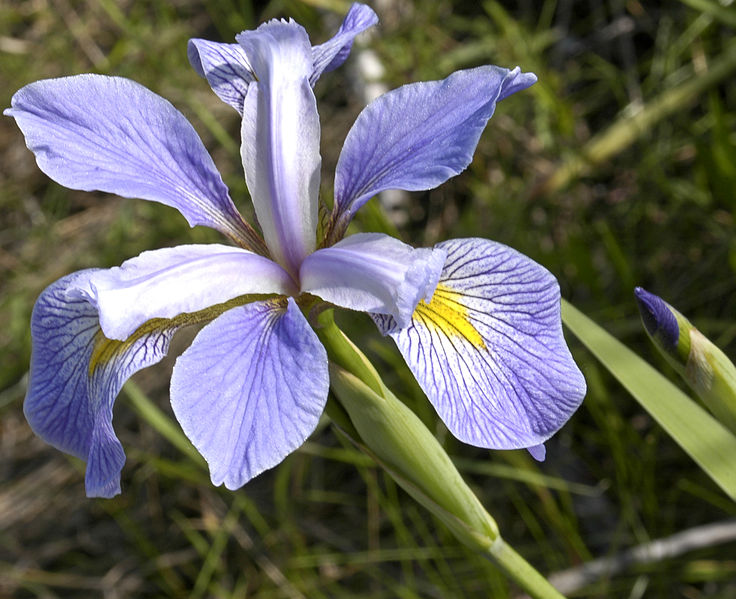
\includegraphics[scale=0.416]{images/virginica.jpg}
\end{center}
{\large \hspace{4.5em} Setosa \hspace{3.3em} Versicolor \hspace{2.5em} Virginica}

\begin{exampleblock}{Задача}
Определить вид ириса на основании длины чашелистика, ширины чашелистика, длины лепестка и ширины лепестка.
\end{exampleblock}

\end{frame}

\begin{frame}{Ирисы Фишера}

\begin{center}
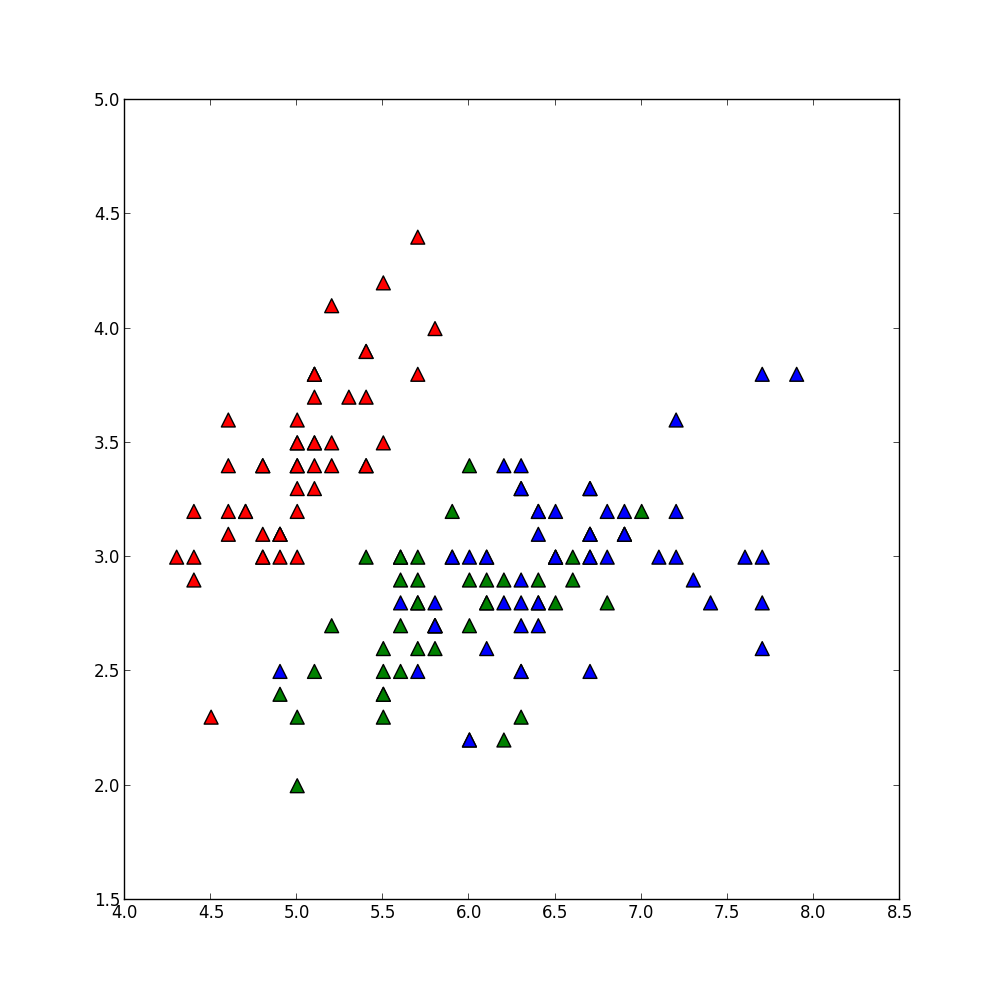
\includegraphics[scale=0.2]{images/iris01.png} \;
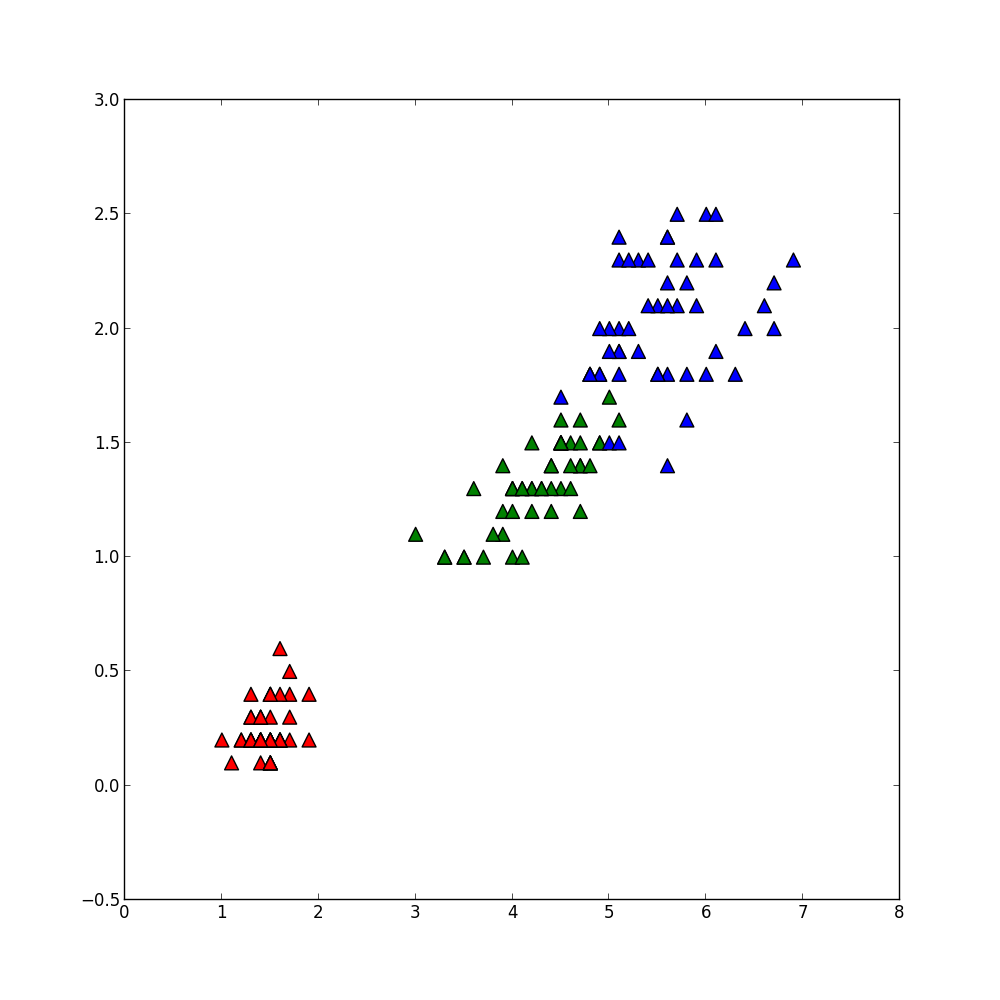
\includegraphics[scale=0.2]{images/iris23.png}
\end{center}

\end{frame}

\begin{frame}{Многомерное нормальное распределение}

\[
\mathcal{N(\mathbf{x} | \mathbf{\mu}, \mathbf{\Sigma}}) = \frac{1}{(2 \pi)^{D/2}} \frac{1}{|\mathbf{\Sigma}|^{1/2}} \exp \left\{-\frac{1}{2}(\mathbf{x} - \mathbf{\mu})^T \Sigma^{-1} (\mathbf{x} - \mathbf{\mu})\right\}
\]

\vspace{0.7em}
\begin{center}
{\bf Параметры}
\end{center}
\quad${D}$-мерный вектор средних\qquad$D \times D$-мерная матрица ковариации 
\[
\mathbf{\mu} = \int \mathbf{x} p({\mathbf{x}}) d\mathbf{x}
\qquad\qquad\qquad
\mathbf{\Sigma} = E[(\mathbf{x} - \mathbf{\mu})(\mathbf{x} - \mathbf{\mu})^T]
\]

\end{frame}

\begin{frame}{Генеративная модель}

Рассматриваем 2 класса
\[
p(y_1 | x) = \frac{p(x | y_1) p(y_1)}{p(x | y_1) p(y_1) + p(x | y_2) p(y_2)} = \frac{1}{1 + e^{-a}} = \sigma(a)
\]
\[
a = \ln \frac{p(x | y_1)p(y_1)}{p(x | y_2)p(y_2)}
\]
$\sigma(a)$ -- сигмоид-функция, $a = \ln (\sigma/(1-\sigma))$

\begin{center}
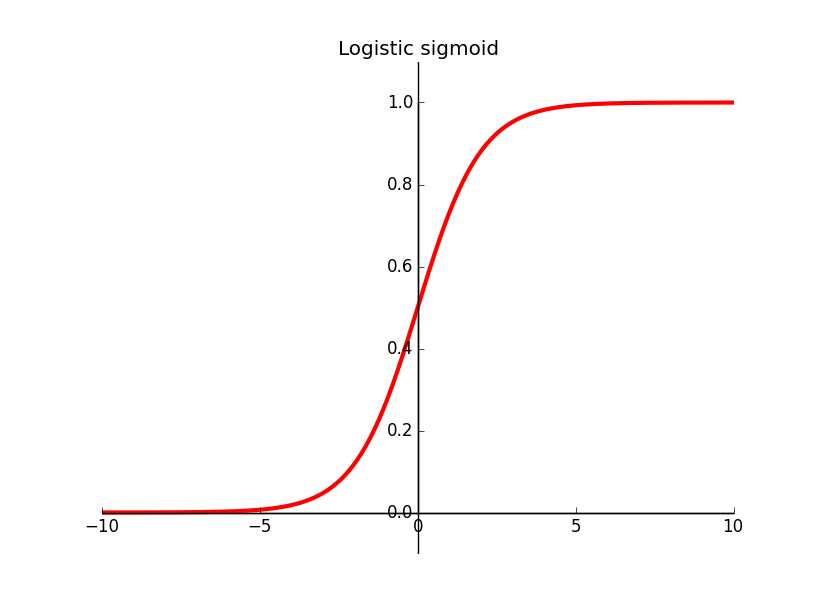
\includegraphics[scale=0.28]{images/sigmoid.png}
\end{center}

\end{frame}

\begin{frame}{Случай нормальных распределений}

Пусть 
\[
p(\mathbf{x} | y_k) = \mathcal{N}(\mathbf{x} | \mathbf{\mu}_k, \mathbf{\Sigma}),
\]
тогда
\[
p(y_1 | \mathbf{x}) = \sigma(\mathbf{w}^T \mathbf{x} + w_0),
\]
где
\[
\mathbf{w} = \mathbf{\Sigma}^{-1} (\mu_1 - \mu_2)
\]
\[
w_0 = - \frac 1 2 \mu_1^T \mathbf{\Sigma}^{-1} \mu_1 + \frac 1 2 \mu_2^T \mathbf{\Sigma}^{-1} \mu_2 + \ln \frac{p(y_1)}{p(y_2)}
\]
Аналогичный результат для любых распределений из экспоненциального семейства

\end{frame}

\begin{frame}{Maximum Likelihood}

\[
p(y_1, \mathbf{x}) = p(y_1) p(\mathbf{x} | y_1) = \pi \mathcal{N}(\mathbf{x} | \mathbf{\mu}_1, \mathbf{\Sigma})
\]
\[
p(y_2, \mathbf{x}) = p(y_2) p(\mathbf{x} | y_2) = (1 - \pi) \mathcal{N}(\mathbf{x} | \mathbf{\mu}_2, \mathbf{\Sigma})
\]
Функция правдоподобия
\[
p(Y, X | \pi, \mu_1, \mu_2, \mathbf{\Sigma}) = \prod_{n=1}^N \left[ \pi \mathcal{N}(\mathbf{x} | \mathbf{\mu}_1, \mathbf{\Sigma}) \right]^{y_n} \left[ (1 - \pi) \mathcal{N}(\mathbf{x} | \mathbf{\mu}_2, \mathbf{\Sigma}) \right]^{1 - y_n} 
\]
Максимизируя $\log p(Y, X | \pi, \mu_1, \mu_2, \mathbf{\Sigma})$, имеем
\[
\pi = \frac 1 N \sum_{n=1}^N y_n = \frac{N_1}{N_1 + N_2},
\]
\[
\mu_1 = \frac{1}{N_1} \sum_{n=1}^N y_n \mathbf{x}_n, \quad
\mu_2 = \frac{1}{N_2} \sum_{n=1}^N (1 - y_n) \mathbf{x}_n,
\]
аналогично для $\mathbf{\Sigma}$

\end{frame}

\begin{frame}{Логистическая регрессия}

{\bf Дано.}
\[
\mathcal{D} = \{\phi_n = \phi(\mathbf{x}_n), y_n\}, \; y_n \in \{ 0,1\}, \; n = 1 \ldots N
\]
{\bf Модель.}
\[
p(y=1 | \phi) = \sigma(\mathbf{w}^\top \phi)
\]
функция правдоподобия (кросс-энтропия)
\[
l(\mathbf{w}) = \log \left[ \prod_{n=1}^N p^{y_n}(y=1 | \phi_n) (1 - p(y=1 | \phi_n))^{1 - y_n}\right] = 
\]
\[
= \sum_{n=1}^N {y_n \log p(y=1 | \phi_n) + (1- y_n) \log (1 - p(y=1 | \phi_n))} = - J_c(\mathbf{w}) \rightarrow \max_{\mathbf{w}}
\]

\end{frame}

\begin{frame}

Градиент
\[
\nabla J_c(\mathbf{w}) = \sum_{n=1}^N (p(y=1 | \phi_n) - y_n) \phi_n
\]
Гессиан
\[
\nabla^2 J_c(\mathbf{w}) = \sum_{n=1}^N p(y=1 | \phi_n) (1 - p(y=1 | \phi_n)) \phi_n \phi_n^T
\]

\end{frame}

\defverbatim[colored]\gd{%
\begin{lstlisting}[tabsize=4,basicstyle=\ttfamily]
function gd(grad, a0, epsilon):
	initialise eta(k)
	k = 0
	a = a0	 
	do:
		k = k + 1
		a = a - eta(k) grad(a)
	until eta(k) grad(a) < epsilon
	return a
\end{lstlisting}
}

\begin{frame}{Градиентный спуск}

\begin{small}
\gd
\end{small}

\end{frame}

\begin{frame}

\begin{center}
   		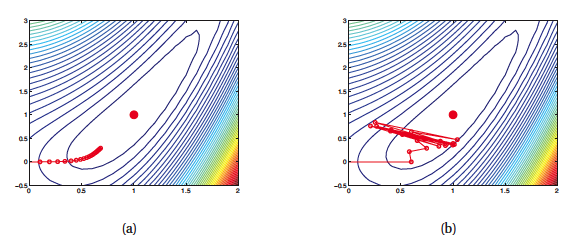
\includegraphics[scale=0.5]{images/gd.png}   		
\end{center}
    
Добавление момента: $\mathbf{a}_{k+1} = \mathbf{a}_k - \eta_k \nabla J (\mathbf{a}_k) + \mu_k (\mathbf{a}_{k} - \mathbf{a}_{k-1})$

\end{frame}

\begin{frame}{Логистическая регрессия: результаты}

	\begin{center}
   		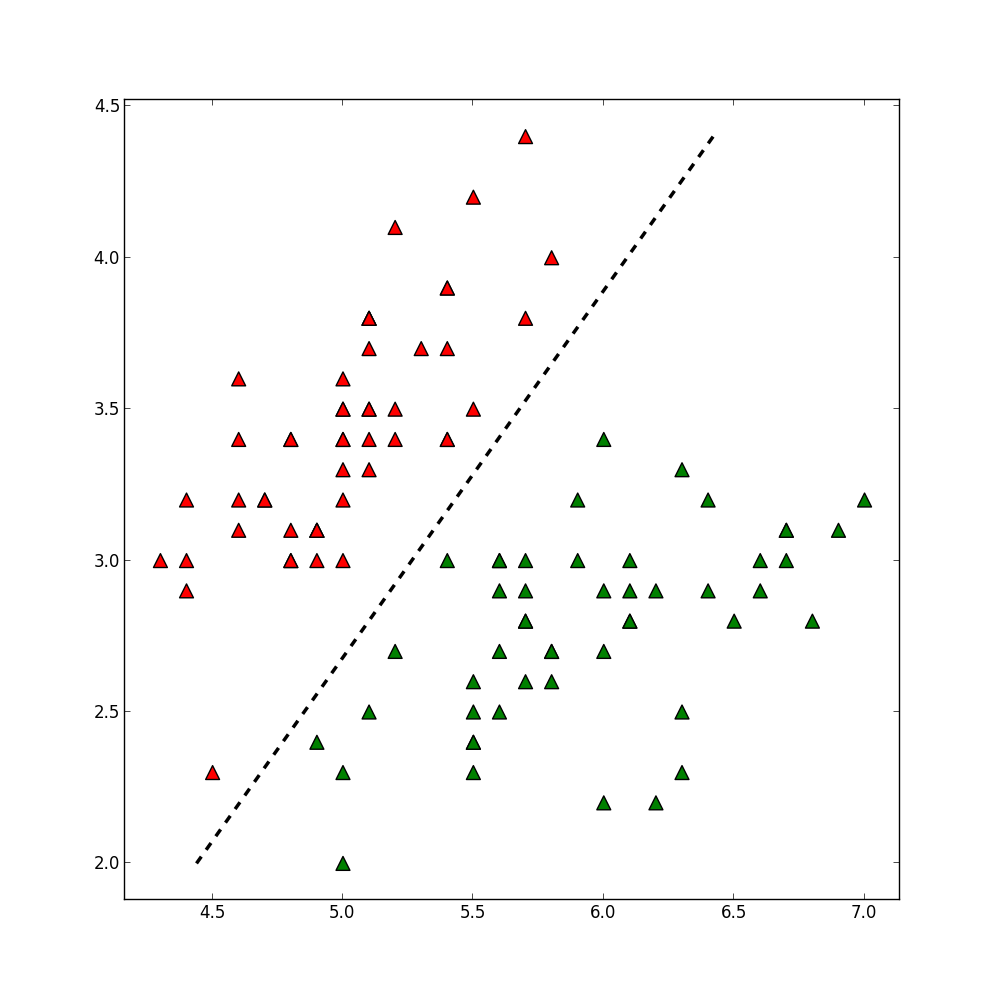
\includegraphics[scale=0.2]{images/lr01.png}\;   		
   		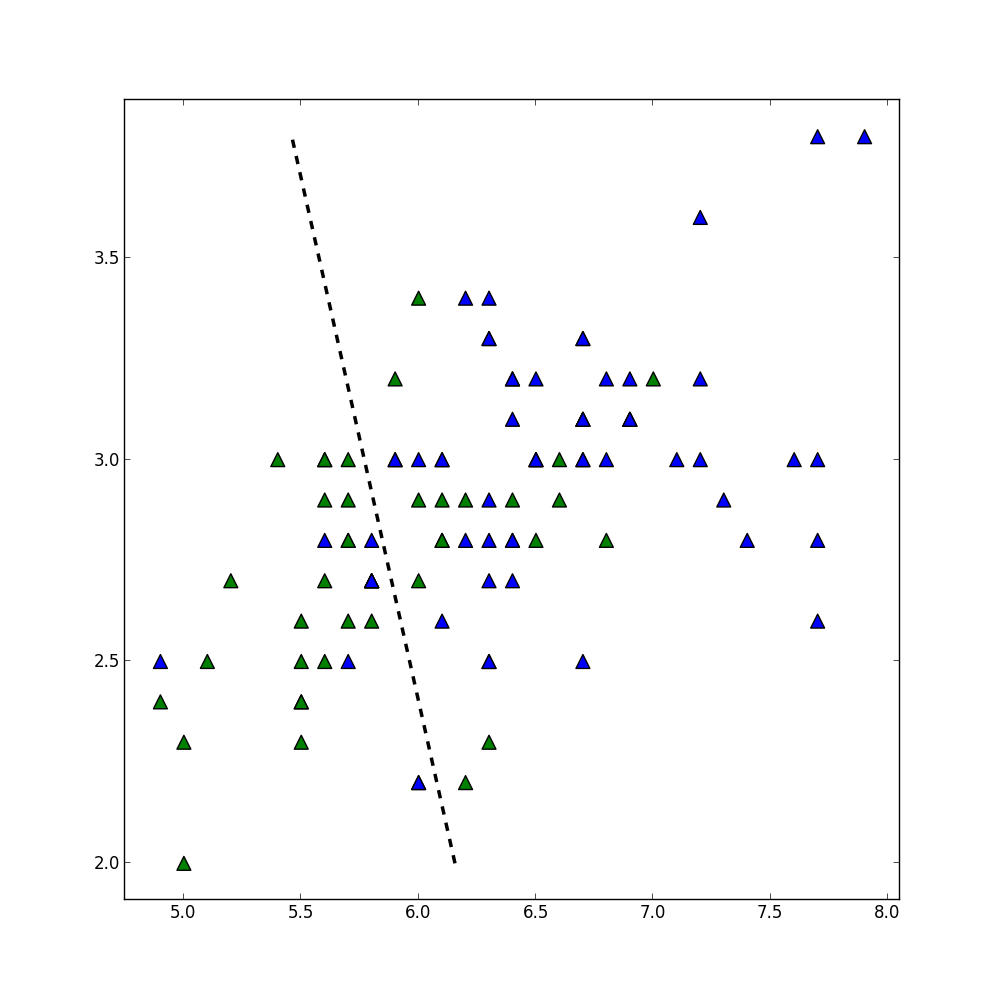
\includegraphics[scale=0.2]{images/lr12.png}
    \end{center}

\end{frame}

\begin{frame}{Обобщенная линеная модель / GLM}

\begin{columns}[T]
    \begin{column}{.5\textwidth}
    \vspace{2em} 
\[
y(\mathbf{x}, \mathbf{w}) \sim pdf\left[ f(\mathbf{w}^\top \phi(\mathbf{x})) \right],
\]
\begin{itemize}
\item $\phi_n(\mathbf{x})$ -- базисные функции
\item $f(a)$ -- функция активации
\item $pdf$ -- распределение из экспоненциального семейства
\end{itemize}

    \end{column}
       
    \begin{column}{.5\textwidth}
    \vspace{-2em}
	\begin{center}
   		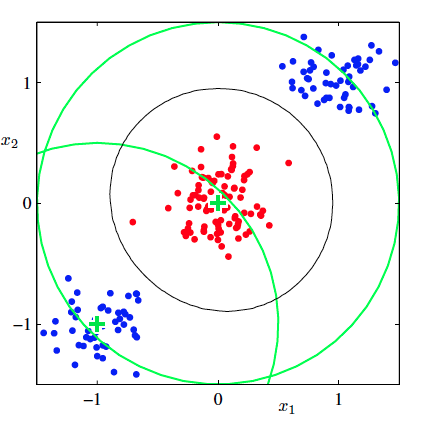
\includegraphics[scale=0.25]{images/nl.png}
   		
   		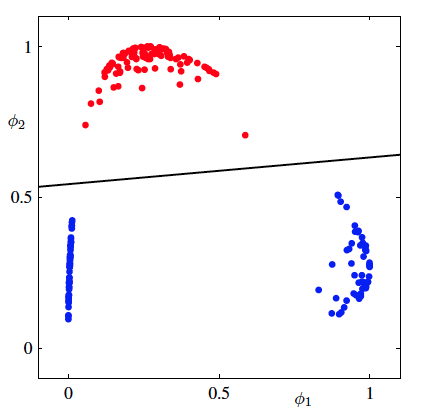
\includegraphics[scale=0.25]{images/l.png}
    \end{center}
    \end{column}
  \end{columns}

\end{frame}

\begin{frame}

\begin{center}
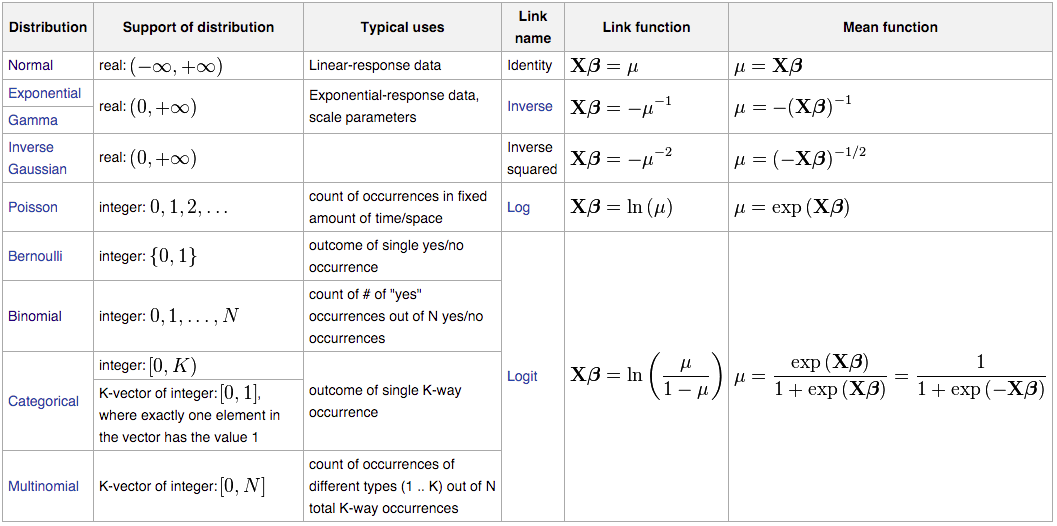
\includegraphics[width=\textwidth]{images/glm.png}
\end{center}

Источник: \href{https://en.wikipedia.org/wiki/Generalized_linear_model}{Wikipedia}

\end{frame}

\begin{frame}{Мультикласс классификация}

\begin{itemize}
\item one-vs-rest \\
{\it Строим $K$ моделей, каждая соответствует одному классу}
\item one-vs-one \\
{\it Строим $K(K-1)/2$ моделей, каждая соответствует паре классов}
\end{itemize}

\end{frame}

\begin{frame}

\begin{center}
\Large Вопросы
\end{center}

\end{frame}

\end{document}